\chapter{Literature Review}
\label{Chapter2}
\lhead{Chapter 2. \emph{Literature Review}}

\section{Optimisation in Air Travel}

\subsection{Airline Scheduling Optimisation}

IN \cite{airline_fleet_assignement}.
\begin{itemize}
    \item Key driver of the revenue for a company: assign the wrong airport with not the good capacity is not optimised
    \item Complex problem - number of daily flights for a company can be very important
\end{itemize}

\begin{itemize}
    \item Comparison between the traditional apporach and the new apporach
    \item Traditionnal: treated as a standalone problem - assumptions like daily flight at fixedhours - point forecasts for the passenger demand
    \item Modern: integrating the FAP with other airline processes such as maintenance - crew Scheduling problem
\end{itemize}

\subsection{crew scheduling problem} % (fold)
\cite{crew_scheduling_problem}

The crew scheduling problem is defined in this paper where the author emphasises the particularity of this problem compared to the set covering/partitonning problem.

The CSP's goal is to assign crews to a sequence of task with defined start and end times. The goal is to ensure that all crew's member can complete all the tasks, without exceeding a total working time.

According to this report \cite{ryanair_youtube_report} - all the airlines companies deal with crew scheduling and especially the low cost companies because that's how they optimise everything and then become competitive.


\subsection{disruption management} % (fold)
\label{sub:disruption management}

\cite{disruption_management}

Diruption in airlines can occur due to various factor -> crew unavailability, accumulated delay along the day because of air control that compells to cancel or delay flights, weather, mechanical problems ...

Disruption management for airline company is crucial because one flight' schedule is planned several months in advanced \cite{flight_scheduling}, hence the objective is to minimise the impact on flights, passangers, airline operations.
The two mains drivers of disruption management are aircraft recovery and crew recovery.
\begin{itemize}
    \item Aircraft recovery: Reassigning aircraft to flights after disruption by taking care of schedules, airports availibility, maintenance
    \item Crew recovery: reassigning crew members to flights by respecting all flights are staffed appropriattely
\end{itemize}


\subsection{Airline adaptation to new demand} % (fold)
\label{sub:Airline adaptation to new demand}
%\cite{flight_seasonnality_challenges}

Airline schedule also take care of passenegrs demand.%\cite{flight_seasonnality_challenges}


The airline industry is fastly evolving - growing dominance of leisure travel over business travel. It has created a new demand seasonnality especially in Europe -> cairline companies have to handle this seasonnality demand by balancing high peak

\begin{figure}[!ht]
    \centering
    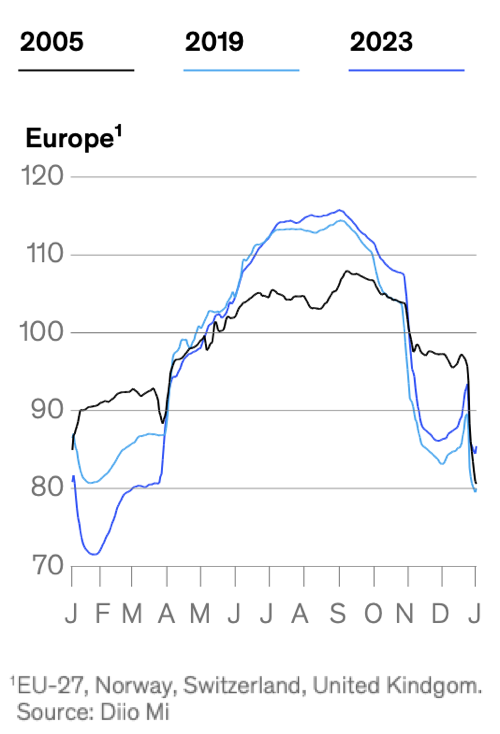
\includegraphics[width=.3\textwidth]{Figures/European Demand.png}
\end{figure}

Demand' seasonnality : airline companies have to adapt
Challenging for airline companies as they have to balance peak seasons with the risk of underutilisation during off-peak times.
Off peak seasons -> planes and crews underused -> driving up costs for passengers but also for the companies

\begin{itemize}
    \item Summer Peak: The airline schedules 65\% more seats in August than in February, deploying more aircraft and crew to meet the demand. Optimization models help the airline decide which routes to prioritize, how many additional flights to add, and how to manage crew rotations to ensure smooth operations despite the high pressure on resources
    \item Winter Through: In winter, the same airline faces low demand, with many aircraft potentially sitting idle. To optimize, the airline might engage in ACMI leasing, reducing its owned fleet temporarily, and outsourcing capacity to adjust dynamically to lower demand. Maintenance activities are ramped up, and crew members are encouraged to take vacations or attend training during this period, optimizing overall productivity.
    \item Revenue Management: Dynamic pricing algorithms adjust fares in real-time based on demand patterns. During summer, prices are optimized to capture the maximum willingness to pay from tourists, while in winter, prices might be adjusted to stimulate demand, filling otherwise empty seats and ensuring higher aircraft utilization.
\end{itemize}

\begin{figure}[!ht]
    \centering
    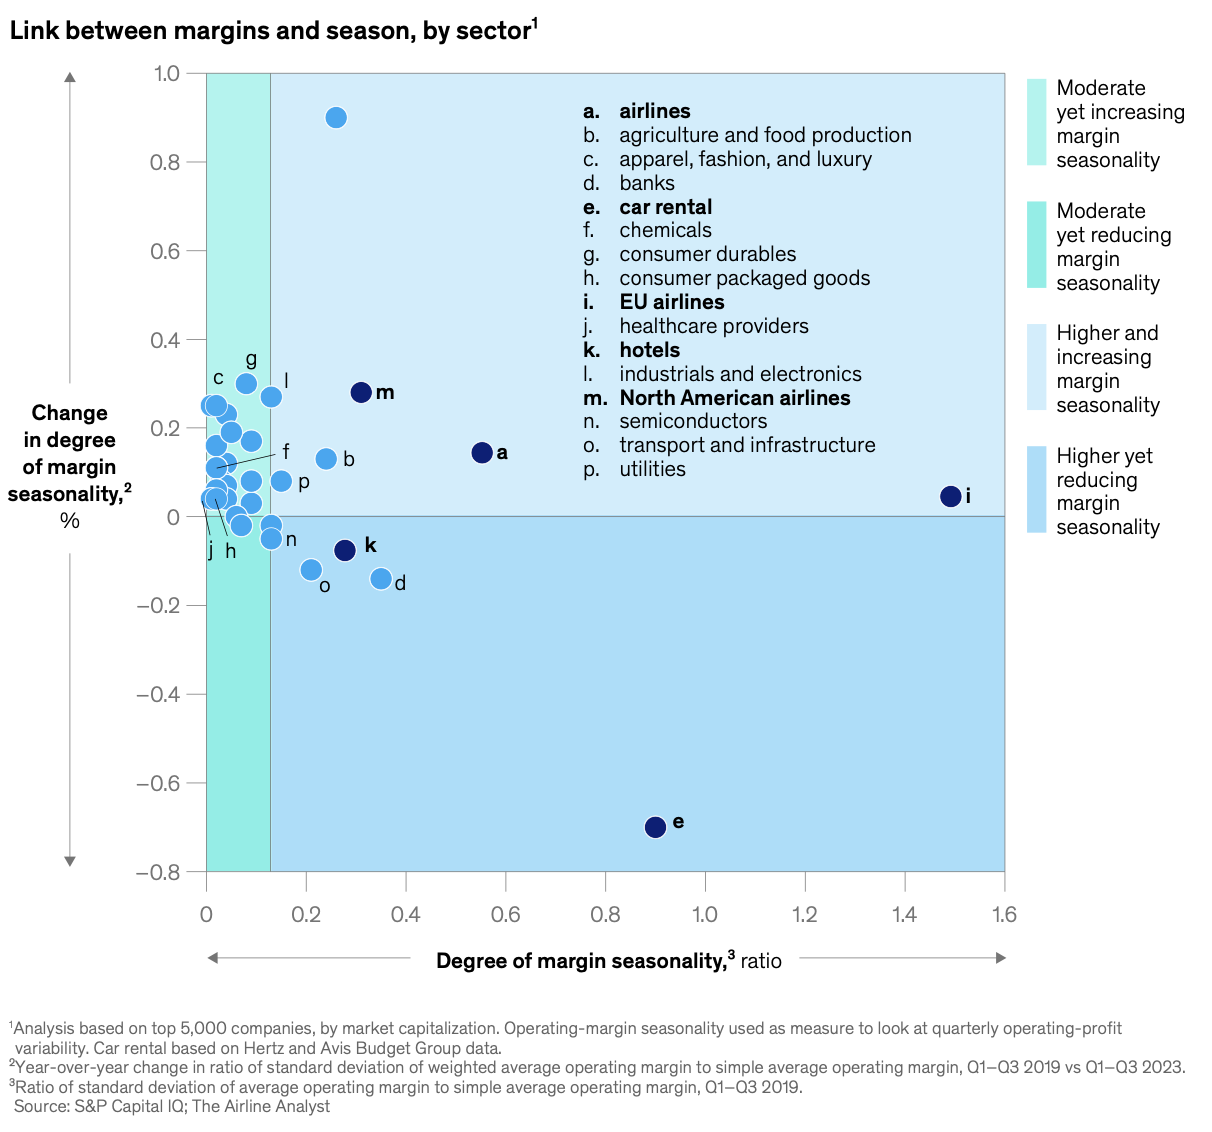
\includegraphics[width=1\textwidth]{Figures/Seasonal margin analysis.png}
    \caption{Compared with other sectors, airlines exhibit a significant and growing link
        between margins and seasons.}
    \label{fig:airline_seasonnality_margin}
\end{figure}


\subsection{Flight connection challenges} % (fold)
\label{sub:Flight connection challenges}

% subsection Flight connection challenges (end)
\newpage
\newpage
\section{Traveling Salesman problem and its adapation}
\cite{np_hardness}

The Traveling Salesman Problem is a well known problem in the Operational Research and Computer Science area. The basic version of the TSP is to find the best roundtrip for a saleman that has to travel around a given number of cities while minimising the overall journey's distance.
This problem is characterised as $\mathcal{NP}$-Hard. This means that there is no known polynomial-time algorithm that can solve all instances of the problem efficiently . In terms of time complexity, if we were to solve it explorating all the possible solutions the time complexity would have been $\mathcal{O}(\frac{(n-1)!}{2})$ where $n$ represents the number of cities.

\begin{figure}[!ht]
    \centering
    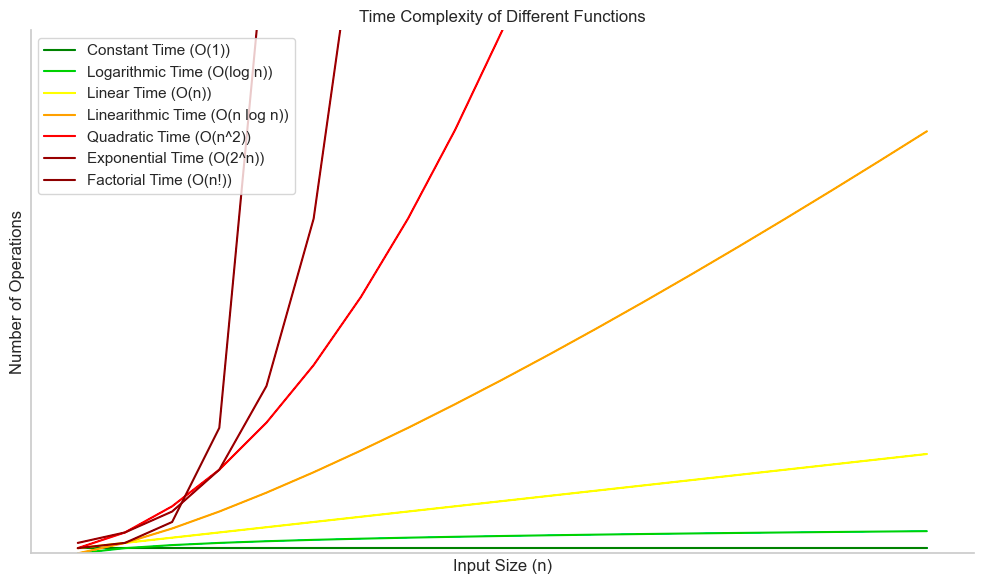
\includegraphics[width=0.8\textwidth]{Figures/NP-hardness - time complexity.png}
    \caption{Time complexity of different functions}
    \label{fig:time_complexity_comparisons}
\end{figure}

On Figure \ref{fig:time_complexity_comparisons}, different time complexity are compared and the factorial time complexity is the worst. That means that these kinds of $\mathcal{NP}$-Hard problem are typically solved using heuristics algorithms. Heuristics solutions do not guarantee to find the absolute optimal solution but can find near-optimal solutions in a much more reasonnable times.
From \cite{time_complexity}

The TSP has been studied a lot, The TSP has been studied a lot, especially because from the TSP il découle de nombreux variantes:

\begin{itemize}
    \item Symmetric TSP (STSP): The distance between cities are symmetric, meaning that the distance to travel from city A to city B is the same as from city B to city A. %\cite{STSP}
    \item Assymetric TSP (ATSP): The distance between cities are assymetric, meaning that the distance to travel from city A to city B is different than the distance to travel from city B to city A.%\cite{ASTP}
    \item Multiple TSP (mTSP): Instead of one salesman, multiple salesman are starting from one city visit all the cities such that each city is visited exactly once. %\cite{mTSP}
    \item Time Window TSP (TWTSP): Each city has to be visited in a defined time slot. %\ref{TWTSP}  
    \item Price-collection TSP (PCTSP): Not all the cities have to be visited, the goal is to to minimise the overall traveler's distance while maximising the price collected earned when visiting a city. %\cite{PCTSP}
    \item Stochastic TSP (STSP): The distances between the cities or the cost of travels are stochastic (\i.e random variables) rather than deterministic. %\cite{Stochastic_TSP}
    \item Dynamic TSP (DTSP): The problem can change over the times, that means that new cities can be added or distances between cities can change while the salesman has already started his journey. %\cite{DTSP}
    \item Generalised TSP (GTSP): The cities are grouped into clusters, the goal is to visit exactly one city from each cluster. %\cite{GTSP}
    \item Open TSP (OTSP): The traveler does not have to end his journey at the starting city. %\cite{OTSP}
\end{itemize}

Multiple algorithms have been developed to address these TSP variants, we can classify them into two major categories:

\begin{itemize}
    \item \textbf{Exact Algorithms}: These algorithms aim to find the optimal solution to the TSP by exploring all possible routes or by using mathematical techniques to prune the search space efficiently. Examples include:
          \begin{itemize}
              \item \textbf{Branch and Bound}: This method systematically explores the set of all possible solutions, using bounds to eliminate parts of the search space that cannot contain the optimal solution. It is often used for smaller instances of TSP due to its computational intensity. %\cite{branch_and_bound}, \cite{branch_and_cut}
              \item \textbf{Cutting Planes}: This technique adds constraints (or cuts) to the TSP formulation iteratively to remove infeasible solutions and converge to the optimal solution. This approach is particularly effective for symmetric TSPs. %\cite{cutting_planes}
              \item \textbf{Dynamic Programming}: Introduced by Bellman, this approach breaks down the TSP into subproblems and solves them recursively, which is highly effective for specific TSP variants, though its complexity grows exponentially. %\cite{dynamic_programming_tsp}
          \end{itemize}
    \item \textbf{Approximation and Heuristic Algorithms}: These algorithms are designed to find near-optimal solutions within a reasonable time frame, especially for large-scale problems where exact methods are computationally infeasible. Examples include:
          \begin{itemize}
              \item \textbf{Greedy Algorithms}: These algorithms make a series of locally optimal choices in the hope of finding a global optimum. An example is the Nearest Neighbor algorithm, which selects the nearest unvisited city at each step. %\cite{greedy}
              \item \textbf{Genetic Algorithms}: Inspired by the process of natural selection, these algorithms evolve a population of solutions over time, using operations such as mutation and crossover to explore the solution space. %\cite{genetic_algorithm}
              \item \textbf{Simulated Annealing}: This probabilistic technique searches for a global optimum by allowing moves to worse solutions based on a temperature parameter that gradually decreases. It is particularly useful for escaping local optima. %cite{simulated_annealing}
              \item \textbf{Ant Colony Optimization}: This metaheuristic is inspired by the foraging behavior of ants and uses a combination of deterministic and probabilistic rules to construct solutions, gradually improving them through pheromone updates. %\cite{ant_colony}
          \end{itemize}
\end{itemize}

Some TSP problems (or its variants) have been solved using other algorithms, hence they are less traditionnal than those mentionned.

\newpage
\section{The Monte Carlo Tree Search algorithm}

The Monte Carlo Tree Search (MCTS) algorithm can be characterised less traditionnal than the previously enounced method in the previous subsection to solve TSP because MCTS is typically used in games.
It is widely use in board games and has been really popular when Google DeepMind developed AlphaGo. AlphaGo is a software that was created to beat the best Go's player in the world.

Go is an ancient board game from China where two players take turns placing black or white stones on a grid. The goal is to capture territory by surrounding empty spaces or the opponent’s stones. Despite its simple rules, Go is incredibly deep and complex, with countless possible moves and strategies. It is known for its balance between intuition and logic, hence it has been a significant focus of artificial intelligence research. \cite{wiki:Go}

In 2016, Lee Sedol \cite{wiki:Lee_Sedol} - the best Go's player in the world has been beaten by AlphaGo 4-1 \cite{alpha_go_documentary}.

MCTS with policy and value networks are at the heart of AlphaGo's decision-making process, enabling AlphaGo's to pick the optimal moves in the complex search of Go. \cite{mcts_alpha_go_algorithm}



\subsection{Overview}
The MCTS' process is conceptually straightforward. A tree is built in an incremental and assymatric manner (Figure \ref{fig:Assymetrical_growth_MCTS}).
For every iteration, a selection policy is used to determine which node we have to select in the tree to perform simulations.
The selection policy balances the exploration  i.e.\ look into part of the tree that have not been visited yet and the exploitation i.e.\ look into part of the trees that appear to be promising.
Once the node is selected, a simulation i.e.\ a statiscally biased sequence is applied from this node until a terminal condition is reached e.g\ no further actions are possible. \cite{mcts_various_policies}

\begin{figure}[!ht]
    \centering
    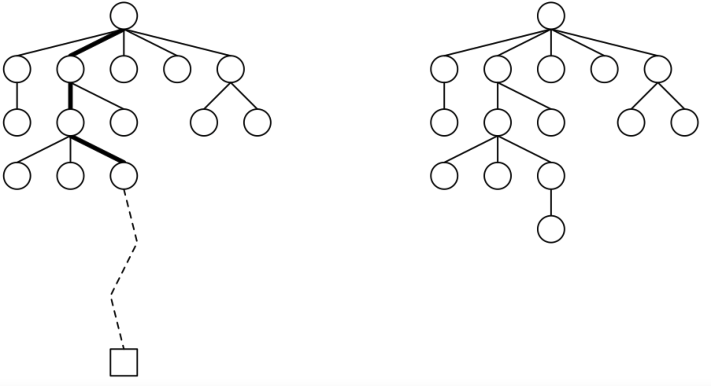
\includegraphics[width=0.5\textwidth]{Figures/assymetric_growth_mcts_tree.png}
    \caption{Assymetrical growth of MCTS - Simulation and Expansion - \cite{mcts_assymetrical_growth}}
    \label{fig:Assymetrical_growth_MCTS}
\end{figure}
To ensure that the reader understands the various stages of the Monte Carlo Tree Search Algorithm, we will begin by looking at a detailed example. This example will illustrate each component of the algorithm in action. We will then generalise the principles discussed, as the basic methodology of this paper is based on the application of the MCTS algorithm.
\newpage


\subsection{Example }
\label{Example}
Let's say we are given a maximisation problem. When starting the game, you have two possible actions $a_1$ and $a_2$ from $S^{0,0}_0$ in the tree $\mathcal{T}$.
Every node is defined like so: $S^{n_i,t_i}_i$ where $n_i$ represents the number of times node $i$ has been visited, $t_i$ the total score of this node.
Furthermore, for every node - we can compute the $UCB1$ value: $UCB1(S^{n_i,t_i}_i)=\bar{V_i} + 2 \sqrt{\frac{\ln N}{n_i}}$ where $\bar{V_i}=\frac{n_i}{t_i}$ represents the average value of the node, $n_i$ the number of times node $i$ has been visited, $N=n_0$ the number of times the root node has been visited/the number of iterations.

Before the first iteration, none node have been visited - $\forall i \in \mathcal{T}, S^{0,0}_{i}$.
\begin{figure}[!ht]
    \centering
    \begin{tikzpicture}[
            root_node/.style={circle, draw=orange!60, fill=orange!5, very thick, minimum size=40},
            visited_node/.style={circle, draw=green!60, fill=green!5, very thick, minimum size=40},
            unvisited_node/.style={circle, draw=gray!60, fill=gray!5, very thick, minimum size=40},
            target_node/.style={circle, draw=green!60, fill=green!5, very thick, minimum size=40},
        ]

        \node[root_node](Root){$S^{0,0}_0$};
        \node[unvisited_node, below left=of Root](S1){$S^{0,0}_1$};
        %\node[target_node, below=of S1, yshift=-1.7cm](Target){};
        \node[unvisited_node, below right=of Root](S2){$S^{0,0}_2$};

        \draw[->] (Root) -- (S1) node[midway, above, xshift=-2mm] {$a_1$};
        \draw[->] (Root) -- (S2) node[midway, above, xshift=2mm] {$a_2$};

        %\draw[->, very thick, decorate, decoration={snake, amplitude=.7mm, segment length=3mm}] (S1) -- (Target);
    \end{tikzpicture}
    \caption{Selection - $I1$}
    \label{fig:Expansion of the tree from the root node}
\end{figure}
At the beginning of $I1$, we then have to choose between these two child nodes (or choose between taking $a_1$ or $a_2$). We then have to calculate the $UCB1$ value for these two nodes and pick the node that maximises the $UCB1$ value (as we are dealing with a maximisation problem).
In Figure \ref{fig:Expansion of the tree from the root node}, neither of these have been visited yet so $USB(S^{0,0}_1)=UCB1(S^{0,0}_2)=\infty$. Hence we decide to choose randomly $S^{0,0}_1$.

$S^{0,0}_1$ is a leaf node that has not been visited - then we can simulate from this node i.e.\ taking random actions from this node to a terminal state as shown on Figure \ref{fig:Simulation - $I1$}:

\begin{figure}[!ht]
    \centering
    \begin{tikzpicture}[
            root_node/.style={circle, draw=orange!60, fill=orange!5, very thick, minimum size=40},
            visited_node/.style={circle, draw=green!60, fill=green!5, very thick, minimum size=40},
            unvisited_node/.style={circle, draw=gray!60, fill=gray!5, very thick, minimum size=40},
            target_node/.style={circle, draw=green!60, fill=green!5, very thick, minimum size=40},
        ]

        \node[root_node](Root){$S^{0,0}_0$};
        \node[unvisited_node, below left=of Root](S1){$S^{0,0}_1$};
        \node[target_node, below=of S1, yshift=-1.7cm](Target){20};
        \node[unvisited_node, below right=of Root](S2){$S^{0,0}_2$};

        \draw[->] (Root) -- (S1) node[midway, above, xshift=-2mm] {$a_1$};
        \draw[->] (Root) -- (S2) node[midway, above, xshift=2mm] {$a_2$};

        \draw[->, very thick, decorate, decoration={snake, amplitude=.7mm, segment length=3mm}] (S1) -- (Target);
    \end{tikzpicture}
    \caption{Simulation - $I1$}
    \label{fig:Simulation - $I1$}
\end{figure}

\newpage
The terminal state has a value of 20, we can write that the rollout/simulation from node $S^{0,0}_1$ node is $\mathcal{R}(S^{0,0}_1)=20$ . The final step of $I1$ is backpropagation. Every node that has been visited in the iteration is updated.
Let $\mathcal{N}_{\mathcal{R},j}$ be the indexes of the nodes visited during the $j-th$ iteration of the MCTS:
\begin{itemize}
    \item Before backpropagation:
          \begin{equation}
              \forall i \in \mathcal{N}_{\mathcal{R},j}, S^{n_i,t_i}_{i,old}
          \end{equation}

    \item After backpropagation:
          \begin{equation}
              \forall i \in \mathcal{N}_{\mathcal{R},j}, S^{n_i+1,t_i+\mathcal{R}(S^{n_i,t_i}_{i,old})}_{i,new}
          \end{equation}
\end{itemize}

We can then define a Backpropagate function:
\begin{center}
    \centering
    $\begin{array}{ccccc}
            \mathcal{B} & : & \mathcal{N}_{\mathcal{R},j} & \to     & \mathcal{N}_{\mathcal{R},j}                    \\
                        &   & S^{n_i,t_i}_{i}             & \mapsto & S^{n_i+1,t_i+\mathcal{R}(S^{n_i,t_i}_{i})}_{i} \\
        \end{array}$
\end{center}



\newpage
Then, back to our example on Figure \ref{fig:Backpropagation_I1} we update the nodes $\mathcal{B}(S^{0,0}_1)=S^{\mathbf{1},\mathbf{20}}_1$ and $\mathcal{B}(S^{0,0}_0)=S^{\mathbf{1},\mathbf{20}}_0$.
\begin{figure}[!ht]
    \centering
    \begin{tikzpicture}[
            root_node/.style={circle, draw=orange!60, fill=orange!5, very thick, minimum size=40},
            visited_node/.style={circle, draw=green!60, fill=green!5, very thick, minimum size=40},
            unvisited_node/.style={circle, draw=gray!60, fill=gray!5, very thick, minimum size=40},
            target_node/.style={circle, draw=green!60, fill=green!5, very thick, minimum size=40}
        ]

        \node[root_node](Root){$S^{\mathbf{1},\mathbf{20}}_0$};
        \node[unvisited_node, below left=of Root](S1){$S^{\mathbf{1},\mathbf{20}}_1$};
        \node[target_node, below=of S1, yshift=-1.7cm](Target){20};
        \node[unvisited_node, below right=of Root](S2){$S^{0,0}_2$};

        \draw[->] (Root) -- (S1) node[midway, above, xshift=-2mm] {$a_1$};
        \draw[->] (Root) -- (S2) node[midway, above, xshift=2mm] {$a_2$};

        \draw[->, very thick, decorate, decoration={snake, amplitude=.7mm, segment length=3mm}] (Target) -- (S1);
    \end{tikzpicture}
    \caption{Backpropagation - I1}
    \label{fig:Backpropagation_I1}
\end{figure}

The fourth phase of the algorithm have been done for $I1$. We can then start the $2^{nd}$ iteration $I2$.
\begin{figure}[!ht]
    \centering
    \begin{tikzpicture}[
            root_node/.style={circle, draw=orange!60, fill=orange!5, very thick, minimum size=40},
            visited_node/.style={circle, draw=green!60, fill=green!5, very thick, minimum size=40},
            unvisited_node/.style={circle, draw=gray!60, fill=gray!5, very thick, minimum size=40},
            target_node/.style={circle, draw=green!60, fill=green!5, very thick, minimum size=40}
        ]

        \node[root_node](Root){$S^{1,20}_0$};
        \node[unvisited_node, below left=of Root](S1){$S^{1,20}_1$};
        %\node[target_node, below=of S1, yshift=-1.7cm](Target){20};
        \node[unvisited_node, below right=of Root](S2){$\mathbf{S^{0,0}_2}$};

        \node[right=2cm of S2, anchor=west] (UCB1) {$UCB(S^{1,20}_1)=20+2 \sqrt{\frac{\ln1}{1}} = 20$};
        \node[below=0.55cm of UCB1, anchor=south] (UCB2) {$UCB(S^{0,0}_2)=\infty$};

        \draw[->] (Root) -- (S1) node[midway, above, xshift=-2mm] {$a_1$};
        \draw[->] (Root) -- (S2) node[midway, above, xshift=2mm] {$a_2$};

        %\draw[->, very thick, decorate, decoration={snake, amplitude=.7mm, segment length=3mm}] (S1) -- (Target);
    \end{tikzpicture}
    \caption{Selection - I2}
    \label{fig:Selection - I2}
\end{figure}
On Figure \ref{fig:Selection - I2}, we can either choose $a_1$ or $a_2$. When a child node has not been visited yet, you pick this node for the Selection or you can compute the $UCB1$ value, it leads to the same conclusion.

\begin{figure}[!ht]
    \centering
    \begin{tikzpicture}[
            root_node/.style={circle, draw=orange!60, fill=orange!5, very thick, minimum size=40},
            visited_node/.style={circle, draw=green!60, fill=green!5, very thick, minimum size=40},
            unvisited_node/.style={circle, draw=gray!60, fill=gray!5, very thick, minimum size=40},
            target_node/.style={circle, draw=green!60, fill=green!5, very thick, minimum size=40},
        ]

        \node[root_node](Root){$S^{\mathbf{2},\mathbf{30}}_0$};
        \node[unvisited_node, below left=of Root](S1){$S^{1,20}_1$};

        \node[unvisited_node, below right=of Root](S2){$S^{\mathbf{1},\mathbf{10}}_2$};
        \node[target_node, below=of S2, yshift=-1.7cm](Target){10};

        \draw[->] (Root) -- (S1) node[midway, above, xshift=-2mm] {$a_1$};
        \draw[->] (Root) -- (S2) node[midway, above, xshift=2mm] {$a_2$};

        \draw[->, very thick, decorate, decoration={snake, amplitude=.7mm, segment length=3mm}] (S2) -- (Target);
    \end{tikzpicture}
    \caption{Simulation and Backpropagation - I2}
    \label{fig:Simulation and Backpropagation - I2}
\end{figure}
\newpage
We can then simulate (Figure \ref{fig:Simulation and Backpropagation - I2}) from the chosen node $S^{0,0}_{2}$ and $\mathcal{R}(S^{0,0}_{2})=10$ and backpropagate all the visited nodes: $\mathcal{B}(S^{0,0}_{2})=S^{1,10}_{2}$ and $\mathcal{B}(S^{1,20}_{0})=S^{2,30}_{0}$.
We now start the $3^{rd}$ iteration, based on the $UCB1$ score we decide to choose $a_1$.
\begin{figure}[!ht]
    \centering
    \begin{tikzpicture}[
            root_node/.style={circle, draw=orange!60, fill=orange!5, very thick, minimum size=40},
            visited_node/.style={circle, draw=green!60, fill=green!5, very thick, minimum size=40},
            unvisited_node/.style={circle, draw=gray!60, fill=gray!5, very thick, minimum size=40},
            target_node/.style={circle, draw=green!60, fill=green!5, very thick, minimum size=40},
        ]

        \node[root_node](Root){$S^{2,30}_0$};
        \node[unvisited_node, below left=of Root](S1){$S^{1,20}_1$};

        \node[unvisited_node, below right=of Root](S2){$S^{1,10}_2$};
        %\node[target_node, below=of S2, yshift=-1.7cm](Target){10};
        \node[right=5mm of S2, anchor=west, yshift=2mm] (UCB1) {$UCB1(S^{1,20}_1)=\mathbf{21.67}$};
        \node[below=0.55cm of UCB1, anchor=south] (UCB2) {$UCB1(S^{1,10}_2)=11.67$};

        \draw[->] (Root) -- (S1) node[midway, above, xshift=-2mm] {$a_1$};
        \draw[->] (Root) -- (S2) node[midway, above, xshift=2mm] {$a_2$};

        %\draw[->, very thick, decorate, decoration={snake, amplitude=.7mm, segment length=3mm}] (S2) -- (Target);
    \end{tikzpicture}
    \caption{Selection - I3}
    \label{fig:Selection - I3}
\end{figure}


$S^{1,20}_{1}$ is a leaf node and has been visited so we can expand this node.

\begin{figure}[!ht]
    \begin{tikzpicture}[
            root_node/.style={circle, draw=orange!60, fill=orange!5, very thick, minimum size=40},
            visited_node/.style={circle, draw=green!60, fill=green!5, very thick, minimum size=40},
            unvisited_node/.style={circle, draw=gray!60, fill=gray!5, very thick, minimum size=40},
            target_node/.style={circle, draw=green!60, fill=green!5, very thick, minimum size=40},
        ]

        \node[root_node](Root){$S^{3,30}_0$};
        \node[unvisited_node, below left=of Root](S1){$S^{2,20}_1$};
        \node[unvisited_node, below right=of Root](S2){$S^{1,10}_2$};
        \node[unvisited_node, below left=of S1](S3){$S^{1,0}_3$};
        \node[unvisited_node, below right=of S1](S4){$S^{0,0}_4$};

        \node[left=8mm of S1, anchor=east] (UCB1) {$UCB1(S^{2,20}_1)=11.48$};
        \node[below=0.55cm of UCB1, anchor=south] (UCB2) {$UCB1(S^{1,10}_2)=\mathbf{12.10}$};

        %\node[target_node, below=of S3, yshift=-1.7cm](Target){0};

        \draw[->] (Root) -- (S1) node[midway, above, xshift=-2mm] {$a_1$};
        \draw[->] (Root) -- (S2) node[midway, above, xshift=2mm] {$a_2$};
        \draw[->] (S1) -- (S3)   node[midway, above, xshift=-2mm] {$a_3$};
        \draw[->] (S1) -- (S4)   node[midway, above, xshift=2mm] {$a_4$};
        %\draw[->, very thick, decorate, decoration={snake, amplitude=.7mm, segment length=3mm}] (S3) -- (Target);
    \end{tikzpicture}
    \caption{Selection and Expansion - I3}
\end{figure}
\newpage
Based on $UCB1$ score we decide to simulate from $S^{0,0}_3$ on Figure \ref{fig:Simulation and Backpropagation - I3}
\begin{figure}[!ht]
    \centering
    \begin{tikzpicture}[
            root_node/.style={circle, draw=orange!60, fill=orange!5, very thick, minimum size=40},
            visited_node/.style={circle, draw=green!60, fill=green!5, very thick, minimum size=40},
            unvisited_node/.style={circle, draw=gray!60, fill=gray!5, very thick, minimum size=40},
            target_node/.style={circle, draw=green!60, fill=green!5, very thick, minimum size=40},
        ]

        \node[root_node](Root){$S^{\mathbf{3},30}_0$};
        \node[unvisited_node, below left=of Root](S1){$S^{\mathbf{2},20}_1$};
        \node[unvisited_node, below right=of Root](S2){$S^{\mathbf{2},10}_2$};
        \node[unvisited_node, below left=of S1](S3){$S^{\mathbf{1},0}_3$};
        \node[unvisited_node, below right=of S1](S4){$S^{0,0}_4$};

        \node[target_node, below=of S3, yshift=-1.7cm](Target){0};

        \draw[->] (Root) -- (S1) node[midway, above, xshift=-2mm] {$a_1$};
        \draw[->] (Root) -- (S2) node[midway, above, xshift=2mm] {$a_2$};
        \draw[->] (S1) -- (S3)   node[midway, above, xshift=-2mm] {$a_3$};
        \draw[->] (S1) -- (S4)   node[midway, above, xshift=2mm] {$a_4$};
        \draw[->, very thick, decorate, decoration={snake, amplitude=.7mm, segment length=3mm}] (Target) -- (S3);
    \end{tikzpicture}
    \caption{Simulation and Backpropagation - I3}
    \label{fig:Simulation and Backpropagation - I3}
\end{figure}
\newpage
Let's do the fourth iteration $I4$ represented on Figure \ref{fig:Selection - Simulation - Backpropagation - I4}:
\begin{figure}[!ht]
    \centering
    \begin{tikzpicture}[
            root_node/.style={circle, draw=orange!60, fill=orange!5, very thick, minimum size=40},
            visited_node/.style={circle, draw=green!60, fill=green!5, very thick, minimum size=40},
            unvisited_node/.style={circle, draw=gray!60, fill=gray!5, very thick, minimum size=40},
            target_node/.style={circle, draw=green!60, fill=green!5, very thick, minimum size=40},
        ]

        \node[root_node](Root){$S^{\mathbf{4,44}}_0$};
        \node[unvisited_node, below left=of Root](S1){$S^{2,20}_1$};
        \node[unvisited_node, below right=of Root](S2){$S^{\mathbf{2},\mathbf{24}}_2$};
        \node[unvisited_node, below left=of S1](S3){$S^{1,0}_3$};
        \node[unvisited_node, below=of S1](S4){$S^{0,0}_4$};
        \node[unvisited_node, below left=of S2](S5){$S^{\mathbf{1},\mathbf{14}}_5$};
        \node[unvisited_node, below right=of S2](S6){$S^{0,0}_6$};


        \node[target_node, below=of S5, yshift=-1.7cm](Target){14};

        \draw[->] (Root) -- (S1) node[midway, above, xshift=-2mm] {$a_1$};
        \draw[->] (Root) -- (S2) node[midway, above, xshift=2mm] {$a_2$};
        \draw[->] (S1) -- (S3)   node[midway, above, xshift=-2mm] {$a_3$};
        \draw[->] (S1) -- (S4)   node[midway, above, xshift=3mm] {$a_4$};
        \draw[->] (S2) -- (S5) node[midway, above, xshift=-2mm] {$a_5$};
        \draw[->] (S2) -- (S6) node[midway, above, xshift=2mm] {$a_6$};

        \draw[->, very thick, decorate, decoration={snake, amplitude=.7mm, segment length=3mm}] (S5) -- (Target);
    \end{tikzpicture}
    \caption{Selection - Simulation - Backpropagation - I4}
    \label{fig:Selection - Simulation - Backpropagation - I4}
\end{figure}

If we were to stop at this stage of the algortihm, the best action to undertake is $a_2$ because it has the higher average value: $\bar{V_1}=\frac{20}{2} \le \bar{V_2}=\frac{24}{2}$.

\section{Driving Factors}